% ---------------------------------------------------------------------
% ---------------------------------------------------------------------
% ---------------------------------------------------------------------

\chapter[Validation of the sparse \textit{N}-PLS method and sNPLS package]{Validation of the sparse \textit{N}-PLS method and sNPLS package}
\label{chapter:validation}
In order to show and assess the performance of our sparse $N$-PLS model, we performed different validations to evaluate its properties regarding prediction accuracy and variable selection capabilities in different scenarios. We also wanted to assess the usability of our package in a real-world data set analysis. For this, simulated and real data sets were used, where we also compared the performance of $N$-PLS against the performance of sparse $N$-PLS regarding predictive capability.


% ---------------------------------------------------------------------
% ---------------------------------------------------------------------
\section{Random synthetic data sets}
The performance of our implementation of the sparse $N$-PLS was first tested using data simulation. In total, fourteen different scenarios with different signal-to-noise ratios and different distributions of the data were assessed. Tuning of the hyperparameters of the models was performed with the \texttt{repeat\_cv} function using 20 repetitions of 10-fold cross-validation following the methodology presented in \autoref{chapter:package}. Each simulation generated a three-way \textbf{\underline{X}} array with $I$=50 samples, $J$=50 variables and $K$=3 times, where variables were randomly sampled from different kinds of distributions (Poisson, Normal and Uniform) with varying parameters as follows:

\vspace{15pt}
\begin{enumerate}
    \item If Normal: $\mathcal{X}\ {\raise.17ex\hbox{$\scriptstyle\sim$}}\ \mathcal{N}(\mu, \sigma)$\ where $\mu\ {\raise.17ex\hbox{$\scriptstyle\sim$}}\ \mathcal{N}(10, 10)$\ and $\sigma\ {\raise.17ex\hbox{$\scriptstyle\sim$}}\ \Gamma(5, 1)$
    \item If Poisson: $\mathcal{X}\ {\raise.17ex\hbox{$\scriptstyle\sim$}}\ \mathcal{P}(\lambda)$\ where $\lambda\ {\raise.17ex\hbox{$\scriptstyle\sim$}}\ \mathcal{N}(10, 2.5)$
    \item If Uniform: $\mathcal{X}\ {\raise.17ex\hbox{$\scriptstyle\sim$}}\ \mathcal{U}(a, b)$\ where $a\ {\raise.17ex\hbox{$\scriptstyle\sim$}}\ \mathcal{N}(10, 10)$\ and $b\ {\raise.17ex\hbox{$\scriptstyle\sim$}}\ \mathcal{N}(100, 10)$
\end{enumerate}
\vspace{10pt}
Only 5 out of the 50 variables were used to construct the response \textbf{\underline{Y}}. They were chosen randomly from the \textbf{\underline{X}} array and assigned randomly the following coefficients: 0.4, 0.5, 0.6, 0.7 and 0.9. In the first run, only one of the three times of the third mode was involved in the creation of, in this case, vector \textbf{y}. In the second run, the three times were involved, but with different coefficients for each variable. In all simulations, random Normal and Poisson errors were added in different amounts to \textbf{y}. For each combination of type and amount of random error, simulations were repeated 100 times. Ability to select the real variables involved in \textbf{y} generation as well as median and 1\textsuperscript{st} and 3\textsuperscript{rd} quartiles of the mean squared error were estimated for each simulation run.

Results of the different simulations carried out on the synthetic data sets are provided in \autoref{table:results_synthetic}. Sparse $N$-PLS outperformed $N$-PLS regarding prediction error, with a mean squared error which was significantly lower in almost all simulation scenarios. This difference in prediction error increased as the signal-to-noise ratio decreased. Regarding variable selection, when performing sparse $N$-PLS, the true variables were almost always included in the selected model. Since simulations were repeated 100 times for each scenario, we summarized their results by giving descriptive statistics of the distribution of the results. Median number of true variables selected in each model was 5 (100\%) in most of the simulations (9 out of 14). In the other 5 simulations, the median number of true variables selected was 4 (80\%). These simulations where one of the true predictor variables was not selected were the ones consisting in the more complex and noisy models, with the three times of the third mode affecting \textbf{y} and lower signal-to-noise ratios. Also, a varying amount of other noise variables were erroneously included in the models. The amount of false positives (noise variables) that were included in the sparse $N$-PLS models increased remarkably as the signal-to-noise ratio of the data decreased, ranging from a median of 2 (4.4\%) in the case of high signal-to-noise ratio data sets, to a median of 7 (15.6\%) noise variables included in the low signal-to-noise, worst-case simulations. 

\begin{table}[hbtp]
\centering
\resizebox{\textwidth}{!}{%
\begin{tabular}{@{}lccccc@{}}
\toprule
\multicolumn{1}{c}{} & \multicolumn{3}{c}{\textbf{Mean Squared Error}}                                                                & \multicolumn{2}{c}{\textbf{Variable selection}}                                                                                                          \\
                     & \textbf{N-PLS}   & \textbf{sNPLS}  & \textbf{\begin{tabular}[c]{@{}c@{}}95\% CI for\\ difference\end{tabular}} & \textbf{\begin{tabular}[c]{@{}c@{}}True variables\\ selected\end{tabular}} & \textbf{\begin{tabular}[c]{@{}c@{}}Noise variables\\ selected\end{tabular}} \\ \midrule
\multicolumn{6}{l}{\textbf{One time}}                                                                                                                                                                                                                                                            \\
Normal error         & 85.58            & 66.23           & \multirow{2}{*}{{[}-21.97, -9.72{]}}                                      & \multirow{2}{*}{5 (5, 5)}                                                  & \multirow{2}{*}{3 (1, 6)}                                                   \\
(sd=1)               & (71.36, 96.24)   & (52.72, 90.54)  &                                                                           &                                                                            &                                                                             \\
Normal error         & 103.16           & 90.71           & \multirow{2}{*}{{[}-16.32, 0.61{]}}                                       & \multirow{2}{*}{5 (5, 5)}                                                  & \multirow{2}{*}{2 (1, 6)}                                                   \\
(sd=1.5)             & (85.98, 114.21)  & (70.54, 121.8)  &                                                                           &                                                                            &                                                                             \\
Normal error         & 116.2            & 99.17           & \multirow{2}{*}{{[}-23.93, -8.02{]}}                                      & \multirow{2}{*}{5 (4.75, 5)}                                               & \multirow{2}{*}{4 (2, 12)}                                                  \\
(sd=2)               & (101.05, 135.47) & (84.34, 121.62) &                                                                           &                                                                            &                                                                             \\
Normal error         & 166.33           & 149.57          & \multirow{2}{*}{{[}-26.84, 2.10{]}}                                       & \multirow{2}{*}{5 (3, 5)}                                                  & \multirow{2}{*}{4 (1, 11)}                                                  \\
(sd=3)               & (134.1, 199.73)  & (117.21, 198.9) &                                                                           &                                                                            &                                                                             \\
Poisson error        & 86.46            & 60.03           & \multirow{2}{*}{{[}-26.66, -9.52{]}}                                      & \multirow{2}{*}{5 (5, 5)}                                                  & \multirow{2}{*}{3 (1, 5)}                                                   \\
(mean=1)             & (70.46, 99.98)   & (45.83, 101.65) &                                                                           &                                                                            &                                                                             \\
Poisson error        & 109.21           & 83.08           & \multirow{2}{*}{{[}-32.09, -16.21{]}}                                     & \multirow{2}{*}{5 (5, 5)}                                                  & \multirow{2}{*}{3 (1, 6)}                                                   \\
(mean=3)             & (92.02, 131.57)  & (67.22, 107.67) &                                                                           &                                                                            &                                                                             \\
Poisson error        & 138.29           & 99.55           & \multirow{2}{*}{{[}-40.58, -21.47{]}}                                     & \multirow{2}{*}{5 (4, 5)}                                                  & \multirow{2}{*}{5 (2, 11)}                                                  \\
(mean=5)             & (108.9, 153.86)  & (78.81, 125.76) &                                                                           &                                                                            &                                                                             \\ \midrule
\multicolumn{6}{l}{\textbf{Three times}}                                                                                                                                                                                                                                                         \\
Normal error         & 165.1            & 107.97          & \multirow{2}{*}{{[}-68.02, -46.07{]}}                                     & \multirow{2}{*}{5 (3, 5)}                                                  & \multirow{2}{*}{5 (2, 11)}                                                  \\
(sd=1)               & (137.81, 202.86) & (91.79, 126.32) &                                                                           &                                                                            &                                                                             \\
Normal error         & 171.95           & 115.75          & \multirow{2}{*}{{[}-69.71, -49.51{]}}                                     & \multirow{2}{*}{5 (3, 5)}                                                  & \multirow{2}{*}{6 (2, 12)}                                                  \\
(sd=1.5)             & (147.6, 206.47)  & (98.58, 133.18) &                                                                           &                                                                            &                                                                             \\
Normal error         & 195.57           & 122.73          & \multirow{2}{*}{{[}-85.29, -59.27{]}}                                     & \multirow{2}{*}{4 (3, 5)}                                                  & \multirow{2}{*}{7 (3, 19)}                                                  \\
(sd=2)               & (159.96, 230.1)  & (100.32, 145.4) &                                                                           &                                                                            &                                                                             \\
Normal error         & 245.71           & 130.97          & \multirow{2}{*}{{[}-125.2, -92.03{]}}                                     & \multirow{2}{*}{4 (3, 4.5)}                                                & \multirow{2}{*}{7 (2, 18)}                                                  \\
(sd=3)               & (199.71, 292.2)  & (107.48, 169.2) &                                                                           &                                                                            &                                                                             \\
Poisson error        & 153.67           & 103.92          & \multirow{2}{*}{{[}-65.17, -45.07{]}}                                     & \multirow{2}{*}{5 (3, 5)}                                                  & \multirow{2}{*}{5 (2, 5)}                                                   \\
(mean=1)             & (135.87, 193.6)  & (85.16, 123.6)  &                                                                           &                                                                            &                                                                             \\
Poisson error        & 186.22           & 115.77          & \multirow{2}{*}{{[}-79.64, -57.47{]}}                                     & \multirow{2}{*}{4 (3, 5)}                                                  & \multirow{2}{*}{6 (3, 13)}                                                  \\
(mean=3)             & (154.9, 213.56)  & (91.33, 134.17) &                                                                           &                                                                            &                                                                             \\
Poisson error        & 205.18           & 118.58          & \multirow{2}{*}{{[}-98.13, -73.24{]}}                                     & \multirow{2}{*}{4 (3, 5)}                                                  & \multirow{2}{*}{6 (3, 15)}                                                  \\
(mean=5)             & (169.3, 236.78)  & (94.83, 140.54) &                                                                           &                                                                            &                                                                             \\ \bottomrule
\end{tabular}%
}
\caption{Results of the analyses performed using N-PLS and sparse N-PLS on the different simulations. Median (1\textsuperscript{st}, 3\textsuperscript{rd} quartile) of the mean squared error and a 95\% confidence interval for the difference in mean squared error between sparse $N$-PLS and $N$-PLS is also provided. True variables selected column indicates the median of the occasions these are included in the models, as well as the 1\textsuperscript{st} and 3\textsuperscript{rd} quartiles (True positives). Noise variables selected column presents analogous results for the Noise variables (False positives)}
\label{table:results_synthetic}
\end{table}

\section{Data driven synthetic data sets}
To further test the performance of the method in selecting highly correlated variables, simulated data resembling the ones of a  toxicogenomics data set \parencite{heijne2004bromobenzene} was analysed. In this work, the effect of the hepatotoxicant bromobenzene in rats was studied. Groups of rats were treated with different doses of this toxic compound dissolved in corn oil for a 48 hours period. At three time points from the start of the treatment, rats were sacrificed. Liver samples were used to extract mRNA for microarray profiling and blood and urine was used for metabolite profiling. Additionally, 21 physiological parameters were recorded: Glucose, A/G ratio, GSH, Body Weight, Creatin, GGT, Urea, Kidneys, Kidney/BW, Triglycerides, Liver, Albumin, Total Protein, ALP, Liver/BW, Bilirubin, LDH, Phospholipids, Cholesterol, ASAT, ALAT. 

For our study, simulated profiles from 14 of these 21 physiological parameters were used to discriminate between two of the different groups (High and Low doses evolution). In order to compute these profiles, since they were not shown in \parencite{heijne2004bromobenzene}, we took advantage of those shown in \cite{conesa2010multiway}, which correspond to the same dataset. 25 samples for high doses and 25 for low doses were simulated, adding to the pattern random normal noise, with standard deviation 0.1.

\autoref{figura29} represents time course levels of the seven patterns corresponding to the 14 physiological parameters evaluated for high and low dose treatment groups. 

\begin{figure}[hbtp]
	\centering
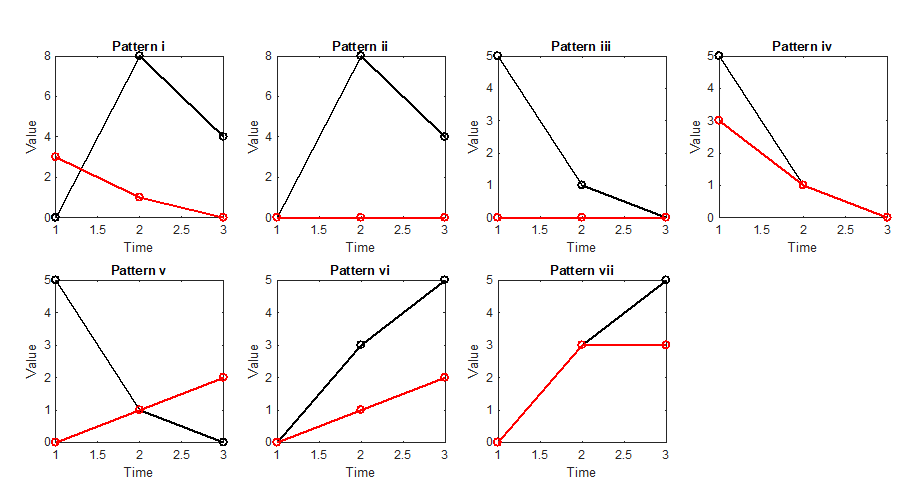
\includegraphics[width=0.7\textwidth]{figura29.png}
\caption{Patterns for the 14 different variables in both groups: High doses (red lines) and low doses (black lines).}
\label{figura29}
\end{figure}

These variables were grouped attending to their common patterns in the following seven groups: i) ALT, AST, LDH and GSH; ii) Creatin and Albumin; iii) Kidney and Cholesterol; iv) Liver, Phospholipids and Triglycerides; v) Glucose; vi) A/G Ratio and vii) Urea.

Our goal with this simulations based on a real data set was to test the ability of the sparse $N$-PLS model in selecting those relevant variables that were associated to the response (discrimination between both groups) even in the case that these variables were correlated. On one hand, since the original lasso for least squares is known to suffer from multicollinearity as explained in \autoref{chapter:modern_techniques}, we were concerned with the performance of our sparse $N$-PLS model in such scenarios. But, on the other hand, since our penalization is included at the model-fitting step of $N$-PLS, which deals excellently with multicollinearity, we were confident that our method would be able to treat correlated variables adequately. More concretely, our expectations were that sNPLS would behave similarly to elastic net, where L1 and L2 penalty are combined \autoref{chapter:modern_techniques}, since PLS is very similar to L2 penalization in the way it shrinks the coefficients \parencite{de1995pls}. Our results, presented in \autoref{table:results_synth2} which summarizes the model coefficients obtained in the analysis, confirmed our hypothesis of good performance in the presence of collinearity. 

\begin{table}[hbtp]
\centering
\begin{tabular}{@{}llll@{}}
\toprule
Variable      & T1 & T2 & T3    \\ \midrule
Glucose       & 0  & 0  & 0     \\
Phospoliphids & 0  & 0  & 0     \\
Kidney        & 0  & 0  & 0     \\
Liver         & 0  & 0  & 0     \\
Cholesterol   & 0  & 0  & 0     \\
Tryglycerids  & 0  & 0  & 0     \\
A/G ratio     & 0  & 0  & 0.077 \\
Urea          & 0  & 0  & 0     \\
Creatinine    & 0  & 0  & 0.082 \\
Albumin       & 0  & 0  & 0.076 \\
ALT           & 0  & 0  & 0.221 \\
AST           & 0  & 0  & 0.221 \\
LDH           & 0  & 0  & 0.221 \\
GSH           & 0  & 0  & 0.101 \\ \bottomrule
\end{tabular}%
\caption{Coefficients of the model}
\label{table:results_synth2}
\end{table}

Overall, results showed good agreement with the structure of the data. All the variables  following the pattern i (i.e., ALT, AST, LDH and GSH) were selected by the method and similar coefficients  were assigned. Additionally, Creatinine and Albumin (pattern ii) were also selected with similar coefficients. Interestingly,  the A/G ratio (pattern vi), a variable uncorrelated to all the others was also selected. However, kidney and cholesterol were not selected by the model, probably because selection was also performed on the third mode and only the third element of the third mode was selected.


\section{Real data sets}
\label{sec:realdata}
Simulated data sets provide a useful suitable first approach to test the performance of the new sNPLS method. However, to exemplify sNPLS and its utility in a more complex context, the proposed method was faced to the analysis of a real dataset, which was derived from a metabolomics study. In metabolomics data sets usually hundreds of variables, with high noise and high correlation, are obtained. This dramatically hinders biomarker discovery and variable selection for predictive models building.  Thus, real processed rat serum samples were used to artificially generate two different groups by adding a set of standards at different final concentrations that additionally showed different trends along time (\autoref{figura30}). In our opinion, this experimental design provides a suitable frame work for assessing sNPLS capabilities when facing real -omics data sets.


\begin{figure}[hbtp]
	\centering
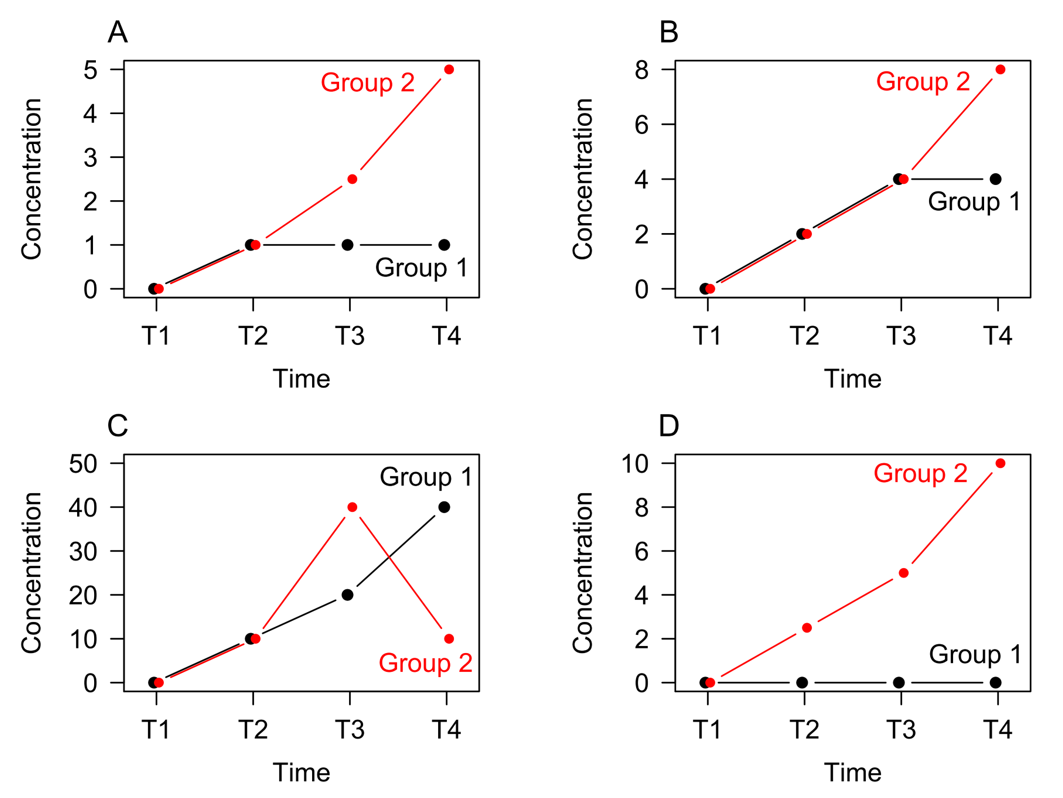
\includegraphics[width=0.7\textwidth]{figura30.png}
\caption{Expected patterns for the four different metabolite classes in group 1 (n=8) and group 2 (n=6).}
\label{figura30}
\end{figure}

In the following paragraphs, the whole experimental procedure for obtaining our real metabolomics data set is thoroughly described. 

Liquid chromatography–mass spectrometry (LC-MS) analyses of rat serum samples were performed in an Agilent 1290 Infinity LC system coupled to an Agilent 6550 Q-TOF mass spectrometer equipped with an ESI source (Agilent Technologies, Santa Clara, CA, USA). LC-MS grade solvents (i.e. water, acetonitrile and methanol) were acquired from Fisher Scientific (Loughborough, UK). All the LC-MS additives and standards were acquired from Sigma–Aldrich/Fluka (Madrid, Spain). Metabolites were separated on an Zorbax SB-Aq column (100 x 2.1 mm; 1.8 {\textmu}m (Agilent Technologies, Santa Clara, CA, USA). Mobile phases consisted of (A) 1mM ammonium fluoride and (B) acetonitrile. The separation was conducted under the following gradient at a flow of 0.3 mL/min: 0 min 3\% (B); 0–2 min 40\% (B); 2-5 min 7\% (B); 5-7 min 50\% (B); 7-12 min 100\% (B); 12-16min 100\% (B); 16-16.5 min 3\% (B); 16.5-18 min 3\% (B). Sample and column temperatures were maintained at 4 ºC and 40ºC, respectively. The injection volume was 5 {\textmu}L. 
The instrument was tuned in the 50-1700 m/z range using an Agilent tune mix in 2GHz extended dynamic range mode (mass resolving power 25,000 FWHM). Detection was performed in ESI (-) mode in the 50-1000 m/z range. A reference solution (m/z 119.0360 and m/z 980.0164) was used to correct small mass drifts during acquisition. The following conditions were employed: capillary voltage, 3.5 kV; nozzle voltage -1.0 kV; fragmentor voltage, 175 V; gas temperature, 200 ºC; drying gas (nitrogen), 14 L/min; nebulizer gas (nitrogen), 35 psi; sheath gas temperature, 350 ºC; and sheath gas flow (nitrogen), 11 L/min. The acquisition rate was set at 4 spectra/s in all cases. Data preprocessing was performed using ProgenesisQI software (Nonlinear Dynamics, UK).

Six-week-old male Oncins France Strain A (OFA) rats (200–240 g) were purchased from Charles River (Barcelona, Spain) and acclimatized to laboratory conditions for at least 7 days. Animals were housed (12-h light-dark cycle, 21–25°C, 30–70\% humidity, woodchip bedding) and fed ad libitum with a standard chow diet (Scientific Animal Food and Engineering, Augy, France). Rats were anesthetized with sodium thiobarbital (0.1 g/kg), and blood was collected by cardiac puncture. After coagulation and centrifugation (1,000 g for 10 min at 4°C), serum samples were aliquoted and stored at - 80°C until the analysis. All the experimental protocols were approved by the Institutional Animal Ethics Committee. 40 {\textmu}L of serum sample were mixed with 120 µL of methanol. After vortexing, samples were kept at -20 ºC for 20 min. Samples were centrifuged (14000 g, 4 ºC, 15 min) and the supernatants transferred to clean tubes and evaporated to dryness. Samples were resuspended in 80 {\textmu}L of water, centrifuged (14000 g, 4 ºC, 5 min), and the clean supernatants transferred to HPLC vials for their LC-MS analysis. Rats serum samples were separated in two groups of sizes 8 and 6 and subsequently fortified with a set of metabolites to generate the patterns already presented in \autoref{figura30}. Metabolites and final concentrations used are summarized in \autoref{table:metabolites}.

\vspace{15pt}
\begin{table}[hbtp]
\centering
\scalebox{0.9}{%
\begin{tabular}{@{}cc@{}}
\toprule
\textbf{Variable Class} & \textbf{Metabolites}                                                                                                                                                                                                                                                                                               \\ \midrule
A                       & \begin{tabular}[c]{@{}c@{}}Capric Acid, Lauric, Acid, Myristic Acid, \\ Myristoleic Acid, Palmitic Acid, \\ Palmitoleic Acid, Octadecanoic Acid, \\ Oleic Acid, Linoleic Acid, Linolenic Acid\end{tabular}                                                                                                         \\ \midrule
B                       & \begin{tabular}[c]{@{}c@{}}Cholic acid, Glycocholic acid, Taurocholic acid, \\ Chenoeoxycholic acid, Glycochenodeoxycholic acid, \\ Taurochenodeoxycholic acid, Deoxycholic acid,\\ Glycodeoxycholic acid, Taurodeoxycholic acid, \\ Lithocholic aid, Glycolithocholic acid, \\ Taurolithocholic acid\end{tabular} \\ \midrule
C                       & \begin{tabular}[c]{@{}c@{}}Valine, Leucine, Isoleucine, Phenylalanine,  \\ Methionine, Cysteine, Proline, Tyrosine,\\ Aspartic acid, Alanine, Glycine, Lysine\end{tabular}                                                                                                                                         \\ \midrule
D                       & \begin{tabular}[c]{@{}c@{}}Ornithine, Glutamate, Glutamine, Citrulline, \\ Arginine, Argininosuccinic Acid, \\ {\textgamma}-glutamyl-glutamic acid, {\textgamma}-glutamyl-glutamine, \\ {\textgamma}-glutamyl-2aminobutyric acid, ophthalmic acid\end{tabular}              \\ \bottomrule
\end{tabular}}
\caption{List of metabolites for each variable class. Metabolites are grouped attending to their physical and chemical properties. Class \textbf{A}, comprises fatty acid; Class \textbf{B}, comprises bile acids; Class \textbf{C}, comprises amino acids; Class \textbf{D} comprises miscellaneous compounds}
\label{table:metabolites}
\end{table}

\subsubsection{Results of the real data set analysis}
Our cross-validation procedure (20 repetitions of 5-fold cross-validation) selected as the optimum parameter values 30 features of \textbf{W}\textsuperscript{J}, 3 features of \textbf{W}\textsuperscript{K} and 2 components. Therefore, 60 variables among the initial 1220 obtained from the LC-MS analysis (30 in each component) were selected by our final sparse $N$-PLS model. Out of the four variable classes which were different between both groups by design (\autoref{table:metabolites}), our model included at least one representative variable for each class. The model also included other variables not present among the four controlled variable classes, but many of them showed similar patterns to those included and could be derivatives or adducts of the original metabolites. Overall, the selection provided by the new model showed a quite feasible result, where not only the real assignable variables (added metabolites) but also those interfering ones could be selected. A list of all the selected variables is presented in \autoref{table:results_real}. The first column list those variables selected by sparse $N$-PLS, while  the second column indicates on which component these variables were selected. The third column shows wether these variables belong or not to one of the classes described in \autoref{table:metabolites}. Finally, column four shows whether those variables that do not belong to any of the assayed classes follows or not a pattern similar to those variables included in \autoref{table:metabolites}. 
\vspace{10pt}
% Please add the following required packages to your document preamble:
% \usepackage{booktabs}
\begin{table}[hbtp]
\centering
\scalebox{0.9}{%
\begin{tabular}{@{}lccc@{}}
\toprule
\textbf{Variable}                                                                                                                                                                             & \textbf{Component} & \textbf{Variable Class} & \textbf{\begin{tabular}[c]{@{}c@{}}Profile similar \\ to class\end{tabular}} \\ \midrule
V8, V16                                                                                                                                                                                       & 1                  & A                       & -                                                                            \\ \midrule
V27, V28, V32                                                                                                                                                                                 & 1                  & B                       & -                                                                            \\ \midrule
V54                                                                                                                                                                                           & 1                  & C                       & -                                                                            \\ \midrule
V58                                                                                                                                                                                           & 2                  & D                       & -                                                                            \\ \midrule
V187, V466, V853                                                                                                                                                                              & 1                  & -                       & A                                                                            \\ \midrule
V470                                                                                                                                                                                          & 1                  & -                       & B                                                                            \\ \midrule
\begin{tabular}[c]{@{}l@{}}V388, V405, V422, V660, \\ V661, V672\end{tabular}                                                                                                                 & 1                  & -                       & C                                                                            \\ \midrule
\begin{tabular}[c]{@{}l@{}}V112, V151, V179, V434, V449,\\ V587, V608, V612, V967, V990\end{tabular}                                                                                          & 2                  & -                       & D                                                                            \\ \midrule
\begin{tabular}[c]{@{}l@{}}V95, V180, V527, V955, V1034,\\ V1056, V1165, V1183, V1512, \\ V2041, V2463, V2520, V2683\end{tabular}                                                             & 1                  & -                       & -                                                                            \\ \midrule
\begin{tabular}[c]{@{}l@{}}V897, V1235, V1322, V1354, \\ V1378, V1389, V1535, V1601, \\ V1627, V1647, V1711, V1715, \\ V1729, V1873, V1935, V1945, \\ V2011, V2077, V2180, V2616\end{tabular} & 2                  & -                       & -                                                                            \\ \bottomrule
\end{tabular}}
\caption{Variables selected by the final sNPLS model and their corresponding assigned variable classes}
\label{table:results_real}
\end{table}




Interestingly, variables of the classes A, B and C and its derivatives or analogues were all exclusively selected in the first component and variables of the class D and its derivatives or analogues were all exclusively selected in the second component. Variables with different patterns to those of the four experimentally generated classes were included in both components, but were more prominent in the second one (13 in the first component versus 20 in the second). 


Finally, the performance of our model was compared with the standard $N$-PLS model. To this end, the metabolomics data set was analyzed using both approaches. The sNPLS model clearly discriminated between the two rat groups (\autoref{figura31}A). However, similar groups’ separation was also obtained by using the standard $N$-PLS (\autoref{figura31}B). The differences between both models appear when comparing \autoref{figura31}B vs \autoref{figura31}G, and \autoref{figura31}C vs \autoref{figura31}H, related to \textbf{W}\textsuperscript{J} and \textbf{W}\textsuperscript{K}, respectively; or \autoref{figura31}D vs \autoref{figura31}I, and \autoref{figura31}E vs \autoref{figura31}J respectively, which are alternative representations. For interpretation purposes, it seems better to compare \autoref{figura31}B vs \autoref{figura31}G for \textbf{W}\textsuperscript{J}, and \autoref{figura31}E vs \autoref{figura31}J for \textbf{W}\textsuperscript{K}. For \textbf{W}\textsuperscript{J}, it seems quite clear that the selection made from sparse $N$-PLS allows a clear interpretation of the metabolites responsible for the separation between the two groups. In the first component, are represented those metabolites belonging to the classes 1, 2 and 3. While, the second component is related to completely independent metabolites (with respect to component one), which could be related to the separation of rats 6 and 13. Many of these metabolites are from class 4, although some of them are not apparently related to any of the designed variable groups.
These interpretations are much more hard to do when using standard $N$-PLS due to the high number of variables to deal with in the second (metabolites) mode, so from this perspective the proposed approach seems to improve the standard $N$-PLS model when trying to directly select the variables of interest (metabolites in this case). However, it should be highlighted that variable selection is out of the $N$-PLS scope. These results shows that when variable selection is of prior relevance for interpretation or validation purposes sparse $N$-PLS come up as a valid alternative
For the interpretation of \textbf{W}\textsuperscript{K}, \autoref{figura31}E and \autoref{figura31}J have been selected. These plots show,  for the first component, a similar pattern, although a slight shift downwards is observed for the standard $N$-PLS. The similar trend observed for both methods strengths the use of the sparse $N$-PLS results, as it provides extra information as discussed above. However, regarding the second component, they do not provided the same result, which could be related to the clear separation of rats 6 and 13 observed in sparse $N$-PLS (\autoref{figura31}A).

\begin{figure}[hbtp]
	\centering
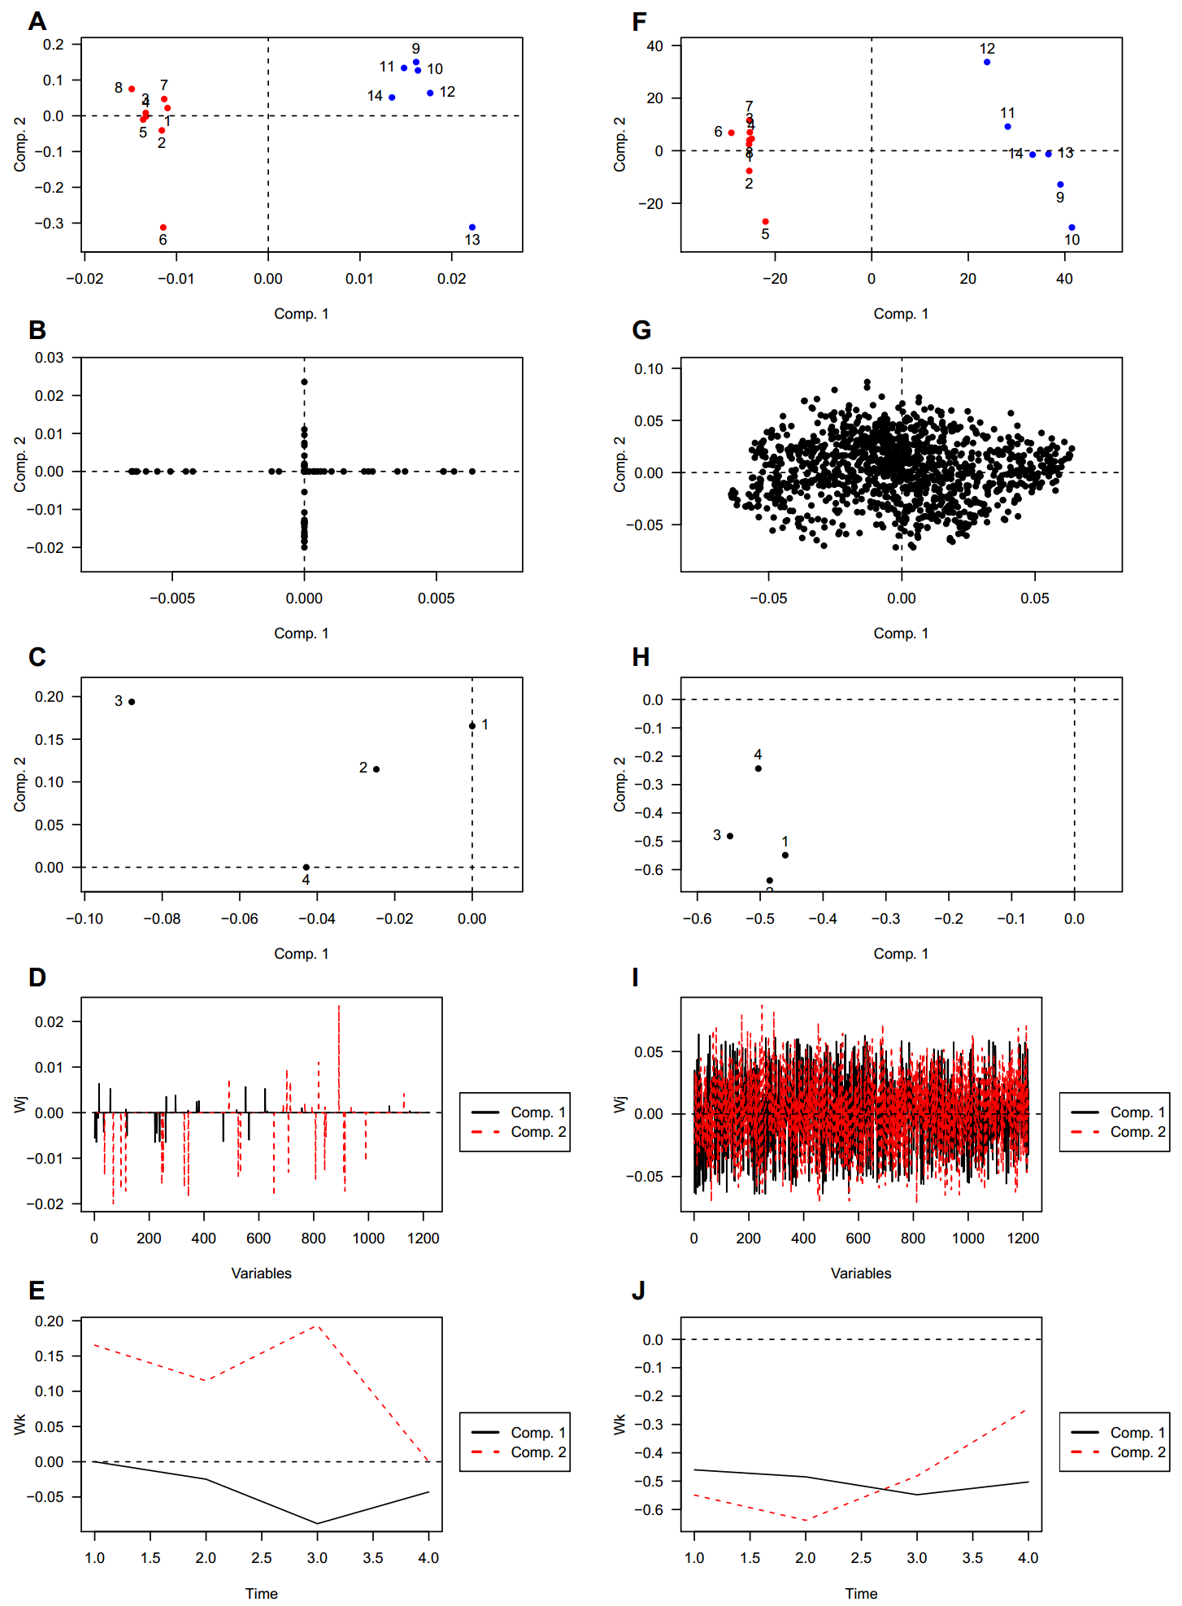
\includegraphics[width=0.91\textwidth]{figura31.png}
\caption{Plots of the sparse $N$-PLS model (left) and the standard $N$-PLS model (right). Score plots of the two first components in the \textbf{T} matrix (A, F); weighting plots of the \textbf{W}\textsuperscript{J} matrix (B, G); weighting plot of the \textbf{W}\textsuperscript{K} matrix (C, H); plots of the loadings of the second (D, I) and third (E, J) modes.}
\label{figura31}
\end{figure}

\section{Comparison with other methods}
As exposed in \autoref{chapter:threeways}, although $N$-PLS does not provide variable selection at the model fitting step, some methods have been developed to perform variable selection after the fitting of the model. Variable Importance in Projection (VIP) scores \parencite{favilla2013assessing} and Selectivity Ratio \parencite{rajalahti2009biomarker} have been used successfully in different studies \parencite{favilla2014ranking, mostafapour2015n, yun2016variable}.

To better get a view of the similarities and differences between our method and the VIP scores and Selectivity Ratio methods, we re-analyzed the real data set presented in \autoref{sec:realdata} with both of them and compared their results with the results presented for sNPLS.
